
% ----------------------------------------------------------------------
%  Set the document class
% ----------------------------------------------------------------------
\documentclass[11pt,a4paper,twoside]{article}

% ----------------------------------------------------------------------
% Define external packages, language, margins, fonts and new commands
% ----------------------------------------------------------------------
%\input{preamble} 
\usepackage[utf8]{inputenc}   % <<<<< Linux
\usepackage[english]{babel} % <<<<< English
\usepackage{notoccite}
\usepackage[skip=0.5\baselineskip]{caption}
\hyphenation{GTKWave}
\usepackage{listings}
\usepackage[all]{nowidow}
\usepackage{float}
%blind text
\usepackage{lipsum}
\usepackage{amsmath} 
\usepackage{graphicx}
\graphicspath{ {./} {../../figlib/}{../mat/}{../sim/} }
\def\FontLn{% 16 pt normal
  \usefont{T1}{phv}{m}{n}\fontsize{16pt}{16pt}\selectfont}
\def\FontLb{% 16 pt bold
  \usefont{T1}{phv}{b}{n}\fontsize{16pt}{16pt}\selectfont}
\def\FontMn{% 14 pt normal
  \usefont{T1}{phv}{m}{n}\fontsize{14pt}{14pt}\selectfont}
\def\FontMb{% 14 pt bold
  \usefont{T1}{phv}{b}{n}\fontsize{14pt}{14pt}\selectfont}
\def\FontSn{% 12 pt normal
  \usefont{T1}{phv}{m}{n}\fontsize{12pt}{12pt}\selectfont}

% Use Arial font as default
%
\renewcommand{\rmdefault}{phv}
\renewcommand{\sfdefault}{phv}
\usepackage{geometry}	
\geometry{verbose,tmargin=2.5cm,bmargin=2.5cm,lmargin=2.5cm,rmargin=2.5cm}

%\usepackage{setspace}
%\renewcommand{\baselinestretch}{1.5}

\usepackage[pdftex]{hyperref} % enhance documents that are to be
                              % output as HTML and PDF
\hypersetup{colorlinks,       % color text of links and anchors,
                              % eliminates borders around links
%            linkcolor=red,    % color for normal internal links
            linkcolor=black,  % color for normal internal links
            anchorcolor=black,% color for anchor text
%            citecolor=green,  % color for bibliographical citations
            citecolor=black,  % color for bibliographical citations
%            filecolor=magenta,% color for URLs which open local files
            filecolor=black,  % color for URLs which open local files
%            menucolor=red,    % color for Acrobat menu items
            menucolor=black,  % color for Acrobat menu items
%            pagecolor=red,    % color for links to other pages
            pagecolor=black,  % color for links to other pages
%            urlcolor=cyan,    % color for linked URLs
            urlcolor=black,   % color for linked URLs
	          bookmarks=true,         % create PDF bookmarks
	          bookmarksopen=false,    % don't expand bookmarks
	          bookmarksnumbered=true, % number bookmarks
	          pdftitle={report},
            pdfauthor={Andre C. Marta},
%            pdfsubject={Thesis Title},
%            pdfkeywords={Thesis Keywords},
            pdfstartview=FitV,
            pdfdisplaydoctitle=true}

\usepackage[numbers,sort&compress]{natbib} % <<<<< References in numbered list [1],[2],...
\usepackage{subcaption} 
\usepackage{mdframed}

%%%%%%%%%%%%%%%%%%%%%%%%%%%%%%%%%%%%%%%%%%%%%%%%%%%%%%%%%%%%%%%%%%%%%%%%
%     Begin Document                                                   %
%%%%%%%%%%%%%%%%%%%%%%%%%%%%%%%%%%%%%%%%%%%%%%%%%%%%%%%%%%%%%%%%%%%%%%%%


\begin{document}

% Set plain page style (no headers, footer with centered page number)
\pagestyle{plain}

% Set roman numbering (i,ii,...) before the start of chapters
%\pagenumbering{roman}

% ----------------------------------------------------------------------
%  Cover page
% ----------------------------------------------------------------------
%%%%%%%%%%%%%%%%%%%%%%%%%%%%%%%%%%%%%%%%%%%%%%%%%%%%%%%%%%%%%%%%%%%%%%%%
%                                                                      %
%     File: Thesis_FrontCover.tex                                      %
%     Tex Master: Thesis.tex                                           %
%                                                                      %
%     Author: Andre C. Marta                                           %
%     Last modified :  2 Jul 2015                                      %
%                                                                      %
%%%%%%%%%%%%%%%%%%%%%%%%%%%%%%%%%%%%%%%%%%%%%%%%%%%%%%%%%%%%%%%%%%%%%%%%

\thispagestyle {empty}

% IST Logo - Signature A
% parameters: bb=llx lly urx ury (bounding box), width=h_length, height=v_length, angle=angle, scale=factor, clip=true/false, draft=true/false. 
\includegraphics[bb=9.5cm 11cm 0cm 0cm,scale=0.29]{IST_A_CMYK_POS}

\begin{center}
%
% Figure (Image or plot)
\vspace{1.0cm}
% height = 50 mm
%\includegraphics[height=50mm]{Figures/Airbus_A350.jpg}

% Title, author and degree
\vspace{1cm}
{\FontLb Circuit Theory and Electronics Fundamentals} \\ % 
\vspace{1cm}
{\FontSn Engineering Physics} \\ % <<<<< EDIT COURSE
\vspace{1cm}
{\FontSn Lab 5: Bandpass filter using OPAMP} \\
\vspace{1cm}
{\FontSn Beatriz Rosalino (96514), Mariana Ribeiro (96552), Sofia Guerreiro (96567)} \\
\vspace{1cm}
{\FontSn 6 June, 2021} \\ % <<<<< EDIT DATE (corresponds to date of oral examination)
%
\end{center}



% ----------------------------------------------------------------------
% Dedication page (optional)
% ----------------------------------------------------------------------
%\input{dedication} 
%\cleardoublepage

% ----------------------------------------------------------------------
%  Acknowledgments (optional)
% ----------------------------------------------------------------------
%\input{acknowledgements}
%\cleardoublepage

% ----------------------------------------------------------------------
%  Abstract (both in English and Portuguese)
% ----------------------------------------------------------------------
%\input{resumo} 
%\cleardoublepage

%\input{abstract} 

% ----------------------------------------------------------------------
%  Table of contents, list of tables, list of figures and nomenclature
% ----------------------------------------------------------------------

% Table of contents
%
\tableofcontents

% List of tables
%\addcontentsline{toc}{section}{\listtablename}
%\listoftables
%\cleardoublepage 

% List of figures
%\addcontentsline{toc}{section}{\listfigurename}
%\listoffigures
%\cleardoublepage 

% Set arabic numbering (1,2,...) after preface
%
%\setcounter{page}{1}
%\pagenumbering{arabic}

% ----------------------------------------------------------------------
%  Body
% ----------------------------------------------------------------------

\section{Introduction}
\label{sec:intro}
The main goal of this work is to analyze an RC circuit and study its various responses to a voltage source that changes over time. First, we studied the behavior of the circuit when the voltage imposed on the capacitor was constant and non zero (Section ~\ref{ssec:tl}), then we studied the natural response of the capacitor (voltage source imposing voltage equal to 0) in (Section ~\ref{ssec:n}), the forced response (voltage source imposing sinusoidal voltage) in (Section ~\ref{ssec:fs}), over time. We also studied the circuit for different frequencies of the sinusoidal signal, plotting the voltages at the capacitor and the nodes of its terminals as functions of frequency Section ~\ref{ssec:freq}.\\

Our circuit (Figure ~\ref{fig:circuit}) consists of 7 resistors, 2 voltage sources - 1 independent, and 1 current controlled dependent one, 1 independent current source and 1 capacitor.\\
The voltage provided by the independent source follows the equation:
\begin{equation}\label{eqn:vss}
\begin{split}
{v_s (t)} = \left\{\begin{array}{ll} \ V_s ,  \quad \ \  if \ \  \ t \leq 0 \\ 
 \ sin(2 \pi f t) , \quad \ \  if \ \ \ t \textgreater 0 \end{array} \right.
  \end{split}
\end{equation}
\begin{figure}[H] \centering
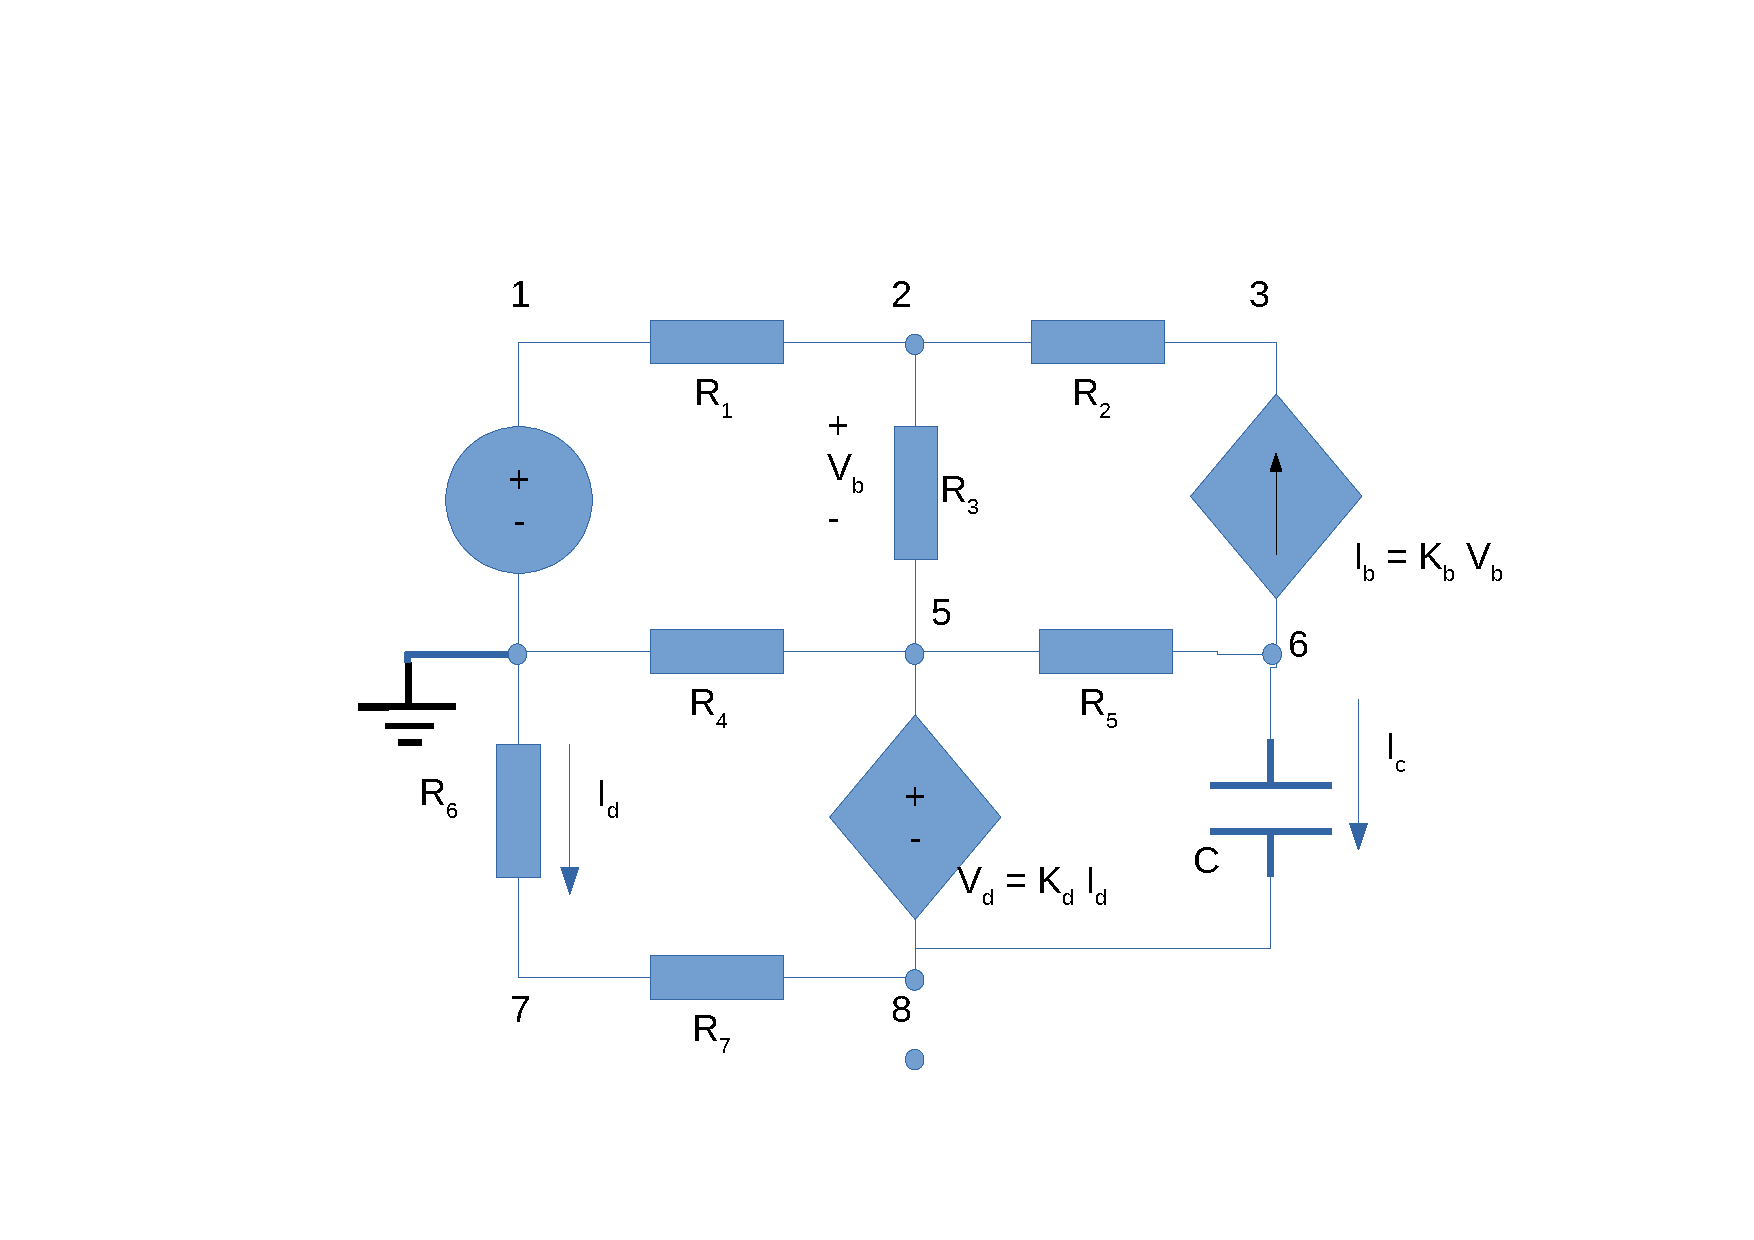
\includegraphics[width=0.8\linewidth]{circuito.pdf}
\caption{Circuit}
\label{fig:circuit}
\end{figure} 
We wrote a system of equations for each theoretical analysis, from Kirchhoff and Ohm's Laws. To get the solutions and plots for these analysis, we used \textit{octave}, which solved our systems of equations efficiently and gave us all currents and voltages for all branches. We then used \textit{ngspice} to get a simulation of this circuit, expecting to obtain the same results. We compared the results from different methods in the conclusion (Section ~\ref{sec:conclusion}).


\section{Simulation}
\label{sec:simulation}
In this circuit, we have a current dependent voltage source between nodes 5 and 8, so that, to sense the controlling current, $I_d$, between nodes GND and 7, we need to use a voltage source of voltage 0V, to sense said current. For this purpose, we placed this source between node 7 and a new node - node 9-, which connects the negative terminal of the voltage source and resistor 7, so that it is in series with resistor 6, through which $I_d$ flows, and therefore senses that same current.\\
\subsection{Operating Point Analysis for t\textless0}
To simulate the response of the circuit for t\textless0, where the voltage source introduces to the circuit a constant voltage, $V_s$, the current through the capacitor is zero, so there is an open circuit between nodes 6 and 8. The results of the operating point analysis for this circuit, t\textless0, obtained using \textit{ngspice}, can be seen in Table (ref).\\

\subsection{Operating Point Analysis for t=0}
To get the operating point analysis for t=0, knowing $v_s(0)=0$, we substitute the capacitor, between nodes 6 and 8, with a voltage source $V_x=V_6-V_8$, where $V_6$ and $V_8$ are the voltage for nodes 6 and 8, respectively, obtained in the previous op analysis (for t\textless0). This is needed so continuity of voltage in the capacitor is guaranteed. The results of this analysis, using \testit{ngspice} can be seen in Table (ref).\\
\subsection{Transient Analysis for Natural Response}
From now on, we have a capacitor in its place, between nodes 6 and 8.\\
To simulate the natural response of the circuit, the source $V_s$ was turned off(the voltage has to be 0V to get the natural response), and we used boundary conditions of $V_6$ and $V_8$(voltages in nodes 6 and 8), as the values obtained in t=0. These conditions will also be used in the latter sections. We did transient analysis, for the [0,20]ms time interval, with a 0.02ms time step. The plot of $v_{6}(t)$ is shown in Figure(ref).\\
\subsection{Analysis of Total Response}
For this section, we now have $V_s$ as a sine wave of frequency f=1k Hz, and amplitude 1 ($V_s=sin(2\pi f t)$). A transient analysis was done, for nodes 6 (V6) and 1 (Vs),again for the [0,20]ms time period with a 0.02ms time step. We can then see the results of the voltage introduced to the circuit (Vs) and the total response on node 6, from both this stimulus from Vs and the natural response of the system. This can be seen in Figure (ref).\\
\subsection{Frequency Analysis}
To evaluate the circuit when the frequency changes, we used ac analysis, by decades - using a frequency logscale. Frequencies were considered from 0.1 Hz to 1MHz and we used 100 points to plot both the magnitude and phase of voltages of nodes 1, 6 and of the capacitor $v_c$, which corresponds to $V_6 - V_8$, as functions of frequency. The magnitude plot can be seen in Figure (ref), and the phase plot in Figure (ref).\\

\section{Theoretical Analysis}
\label{sec:octave}

\subsection{Operating Point Analysis}
The bias circuit-$R_{B1}$, $R_{B2}$ and Vcc- ensures the first transistor is forward-biased. The capacitor $C_1$ causes an open circuit.
We need to define $g_{m1}=I_{C_1}/V_T$, with $V_T=25 \times 10^{-3} V$ and $I_{C_1}=\beta_F (R_{B_2}/(R_{B_1}+R_{B_2})V_{cc} -V_{BEON})/(R_B+(1+\beta_F)R_{E_1})$, where $V_{BEON}=0.7 V$ and $\beta_f=178.7$, $r_{\pi_1}=\beta_F/g_{m1}$ and $r_{o_1}=V_{AFN}/I_{c_1}$, where $V_{AFN}=69.7 V$.
We also replaced the bias circuit with its Thévenin equivalent. Turning off the source Vcc, we get the equivalent resistance $R_B= \frac{1}{\frac{1}{R_{B1}}+\frac{1}{R_{B2}}}$ and since Vcc is in series with both RB1 and RB2, we get the equivalent voltage by voltage divider: $V_{eq}=V_{cc}\frac{R_{B2}}{R_{B1}+R_{B2}}$.
Since $R_{E1}$ and $C_E$ are in parallel with each other, we can also replace them by the equivalent impedance: $Z_{E_1}=\frac{1}{\frac{1}{R_{E_1}}+\frac{1}{Z_{C_E}}}$. For DC analysis, the capacitor is an open circuit, so $Z_{E_1}=R_{E_1}$.

We did operating point analysis using the mesh method, separating the gain stage of the circuit from the output stage. For the gain stage the system of equations is, since $I_{E_1}=I_{B_1}+I_{C_1}$ and $I_{C_1}=\beta_F I_{B_1}$:
\begin{equation}
\left(\begin{array}{ccc} 1 & 0 & 0 \\
R_B & 0 & R_E\\
1 & 1 & -1 \\
\end{array}\right)
\left(\begin{array}{c} I_{B_1} \\ I_{C_1} \\ I_{E_1}  \end{array}\right) 
= \left(\begin{array}{c} \frac{V_{eq}-V_{ON}}{R_B+(1+\beta_F)R_E}\\ 0 \\ -V_{BEON}-V_{eq}  \end{array}\right)
\end{equation},
where $\beta_F$ is the forward common emitter current gain and $V_{BEON}$ is the voltage required for the transistor to be forward biased. \\
With the currents determined we can calculate the nodal voltages of this circuit:
\begin{equation}
    V_1=V_{eq}
\end{equation}
\begin{equation}
    V_2=V_{eq}-R_B I_{B_1}
\end{equation}
\begin{equation}
    V_3=V_{o_{1}}=V_{CC}-R_C I_C
\end{equation}
\begin{equation}
    V_4=V_{cc},
\end{equation}
\begin{equation}
    V_5= V_E=R_E I_{E_1},
\end{equation}
For the output stage, the equation of the super mesh rearranged to get the current in the emitter of the second transistor, $I_{E_{2}}$,  is: 
\begin{equation}
I_{E_2}=\frac{V_{CC}-V_{EBON}-V_I}{R_E}
\end{equation}
Having determined the current $I_{E_2}$ we can calculate $V_{O_2}$:
\begin{equation}
V_{O_2}=V_{CC}-R_E I_{E_2}=V_2
\end{equation}
\begin{equation} 
V_1=V_I
\end{equation}
\begin{equation} 
V_3=V_{cc}
\end{equation}
And the currents are:
\begin{equation}
    I_{C_2}=\beta_F I_{B_2}
\end{equation}
Now $\beta_F=227.3$.
\begin{equation}
    I_{B_2}=I_{E_2}-I_{C_2}
\end{equation}
\begin{figure}[H] \centering
\includegraphics[width=0.8\linewidth]{inc.pdf}
\caption{Gain stage (left) and output stage (right) circuits for DC and incremental analysis}
\label{fig:oc2}
\end{figure} 
\section{Incremental Analysis}
Vcc is now off, since it only has a DC component and this is an AC analysis.
\subsection{Gain stage}
If we turn off $V_S$, we can get an equivalent Thévenin resistance from $R_S$ and $R_B$, $R_{SB}=\frac{1}{\frac{1}{R_S}+\frac{1}{R_B}}$. Since $C_1$ is in series with $R_{SB}$, we can use their equivalent impedance $Z_1=R_{SB}+Z_{C_1}$. For AC analysis, the capacitor is in short circuit, so $Z_1=R_{SB}$.  The output voltage from this part of the circuit is $V_{o_1}=V_5-0$ (Figure 2). Analysing the circuit by mesh analysis, we get that 
\begin{equation}
\left(\begin{array}{ccc}  r_{o_1}+R_C+R_{E_1} & -R_{E_1} & -r_{o_1}\\
-R_{E_1} & R_{E_1}+r_{\pi_1}+R_{BS} & 0\\ 0 & g_{m_1}r_{\pi_1} & 1
\end{array}\right)
\left(\begin{array}{c} I_{A_1} \\ I_{B_1} \\ I_{C_1}  \end{array}\right) 
= \left(\begin{array}{c}  0 \\ v_i \\0 \end{array}\right)
\end{equation}
where $v_i=\frac{R_S}{R_{SB}}v_s$, by voltage divider.
From this we get
\begin{equation}
    I_{A_1}=\frac{R_{E_1}-g_{m_1}r_{\pi_1} r_{o_1}}{(r_{o_1}+R_C+R_{E_1})(R_{BS}+r_{pi_1}+R_{E_1})-g_{m_1}r_{pi_1}R_{E_1}r_{o_1}-R_{E_1}^2}v_i
\end{equation}
We know, from Ohm's law that $v_o=R_C I_{A_1}$, so we have
\begin{equation}
    \frac{v_o}{v_s}=\frac{R_{BS}}{R_S}\frac{R_{E_1}-g_{m_1}r_{\pi_1} r_{o_1}}{(r_{o_1}+R_C+R_{E_1})(R_{BS}+r_{pi_1}+R_{E_1})-g_{m_1}r_{pi_1}R_{E_1}r_{o_1}-R_{E_1}^2}
\end{equation}

The impedance in the source of the circuit, $v_i$ is given, by Ohm's law, by $Z_I=\frac{v_i}{I_{B_1}}$, where from nodal analysis 
\begin{equation}
    I_{B_1}=\frac{R_{E_1}+R_C+r_{o_1}}{(r_{o_1}+R_C+R_{E_1})(R_{BS}+r_{pi_1}+R_{E_1})-g_{m_1}r_{pi_1}R_{E_1}r_{o_1}-R_{E_1}^2}v_i
\end{equation}
so 
\begin{equation}\label{eq:zi}
Z_I=\frac{(r_{o_1}+R_C+R_{E_1})(R_{BS}+r_{pi_1}+R_{E_1})-g_{m_1}r_{pi_1}R_{E_1}r_{o_1}-R_{E_1}^2}{R_{E_1}+R_C+r_{o_1}}
\end{equation}
To calculate the output impedance, we put a voltage test source between nodes 5(Figure 2) and GND of voltage $v_o$, and turn off $v_s$. The impedance here is $Z_o=\frac{v_o}{i_o}$, as seen by the test source. We considered the impedance of the rest of the circuit $Z_X$, so we get that $Z_o=\frac{1}{\frac{1}{Z_X}+\frac{1}{R_C}}$.
Since $R_{B}||r_{\pi_1}$, by voltage divider, $v_\pi=-\frac{r_{\pi}}{R_\pi +R_B}v_4$.
We know, by nodal analysis that 
\begin{equation}
\frac{v_4}{R_{\pi_1}+R_B}-g_{m_1}v_\pi+\frac{v_4}{R_{E_1}}+\frac{v_4}{r_0}-\frac{v_o}{r_o}=0
\end{equation}
And $Z_X=\frac{v_o}{\frac{v_o-v_4}{r_o}+g_{m_1}v_\pi}$.\\
When $R_{E_1}=0$, the circuit seen by the test source is only $R_{C}||r_{o_1}$ and the current source. Therefore, the impedance seen by the test source $Z_0=R_{C}||r_{o_1}$
\subsection{Output Stage}
In this part of the circuit, we can get the conductances for $r_{\pi_2}$, $r_{o_2}$ and $R_{E_2}$:
\begin{equation}
    g_{\pi_2}=\frac{g_{m_2}}{\beta_F}
\end{equation}
where
\begin{equation}
    g_{m_2}=\frac{I_{C_2}}{V_T}
\end{equation}
\begin{equation}
    g_{o_2}=\frac{I_{C_2}}{V_A}
\end{equation}
\begin{equation}
    g_{E_2}=\frac{1}{R_{E_2}}
\end{equation}
Since $R_{E_2}$ and $r_{o_2}$ are in parallel with each other, we can replace them by the equivalent resistance: $R'=\left(\frac{1}{R_{E_2}}+\frac{1}{r_{o_2}}\right)^{-1}$ and get the following node equation:
\begin{equation}\label{eq:bla}
    \left(\frac{1}{R_{E_2}}+\frac{1}{r_{o_2}}\right)v_{o_2}+\frac{v_{o_2}-v_{i_2}}{R_{\pi_2}}-g_{m_2}v_{\pi_2}=0
\end{equation}
Where $v_{\pi_2}=v_{i_2}-v_{o_2}$. From equation~\ref{eq:bla} we get the gain:
\begin{equation}
    A_{v_2}=\frac{v_{o_2}}{v_{i_2}}=\frac{g_{m_2}}{g_{m_2}+g_{\pi_2}+g_{o_2}+g_{E_2}}
\end{equation}
The input impedance is given by:
\begin{equation}
    Z_{i_2}=\frac{v_{i_2}}{i_{i_2}}= \frac{g_{m_2}+g_{\pi_2}+g_{o_2}+g_{E_2}}{g_{\pi_2}(g_{\pi_2}+g_{o_2}+g_{E_2})}
\end{equation}
The output impedance is given by:
\begin{equation}
    Z_{o_2}=\frac{v_{o_2}}{i_{o_2}}= \frac{1}{g_{m_2}+g_{\pi_2}+g_{o_2}+g_{E_2}}
\end{equation}


\subsection{Whole circuit}
\subsection{Frequency Analysis}
\begin{figure}[H] \centering
\includegraphics[width=0.8\linewidth]{gain.pdf}
\caption{Circuit for Frequency analysis}
\label{fig:oc2}
\end{figure} 
Since Vcc is a DC source, it is not taken into account for this analysis.
Since $R_{E1}=100 \Omega$ and $C_E$ are in parallel with each other, we can also replace them by the equivalent impedance: $Z_{E_1}=\frac{1}{\frac{1}{R_{E_1}}+\frac{1}{Z_{C_2}}}$.\\
Since the load and $C_2$ are in series with each other, we can replace them with $Z_2=R_L+Z_{C_2}$. This set is in parallel with $Ro_2$, so we can replace this with its impedance: $Z_3=\frac{1}{\frac{1}{Z_2}+\frac{1}{Ro_2}}$. All of this is also in parallel with the resistor $R_{E_2}$, so the equivalent impedance for all these components is $Z_T=\frac{1}{\frac{1}{R_{E_2}}+\frac{1}{Z_3}}$.
We run nodal analysis to find the voltages of the different nodes:
\begin{equation}
\left(\begin{array}{ccccc} 1 & 0 & 0 & 0 & 0\\ -\frac{1}{Z_1} & \frac{1}{Z_1}+\frac{1}{R_{\pi_1}} & -\frac{1}{R_{\pi_1}} & 0 & 0\\
0 & -\frac{1}{R_{\pi_1}}-gm_1 & \frac{1}{Z_{E_1}}+\frac{1}{R_{\pi_1}}+gm_1+\frac{1}{Ro_1} & -\frac{1}{Ro_1} & 0\\0&  gm_1 & -gm_1-\frac{1}{Ro_1} & \frac{1}{Ro_1}+\frac{1}{R_C}+\frac{1}{R_{\pi_2}} & -\frac{1}{R_{\pi_2}} \\
0 & 0 & 0 & -\frac{1}{R_{\pi_2}} -gm_2 &\frac{1}{Z_T}+\frac{1}{R_{\pi_2}}+gm_2
\end{array}\right)
\left(\begin{array}{c} V_1 \\ V_3 \\ V_4 \\ V_5 \\V_6 \end{array}\right) 
= \left(\begin{array}{c} V_s \\ 0 \\ 0 \\0 \\ 0\end{array}\right)
\end{equation}
The output voltage, on the load is given by $V_{out}=V_6-0$. To calculate the gain, we divide $V_{out}$ by $V_{S}$. We do this for different frequencies, from 10Hz to 100MHz to see how the gain varies with frequency, the frequency response.
\subsection{Input and output impedances}
The input impedance of the circuit is equal to the input impedance of the gain stage, which can be determined by equation ~\ref{eq:zi}. \\
The total output impedance of the circuit is given by:
\begin{equation}
    Z_o =\frac{v_o}{i_o} =\frac{1}{g_{o_2}+\frac{g_{m_2}}{g_{\pi_2}}g_B+g_{E_2}+g_B}
\end{equation}
Where 
\begin{equation}
    g_B=\frac{1}{\frac{1}{g_{\pi_2}}+Z_{o_g}}
\end{equation}
with $Z_{o_g}$ the output impedance of the gain stage.


\section{Results}
\label{sec: res}

\subsection{Plots}
The results obtained from the analysis in Section ~\ref{sec: sim} can be seen in Figure ~\ref{fig:rc1}.
\begin{figure}[H] \centering
  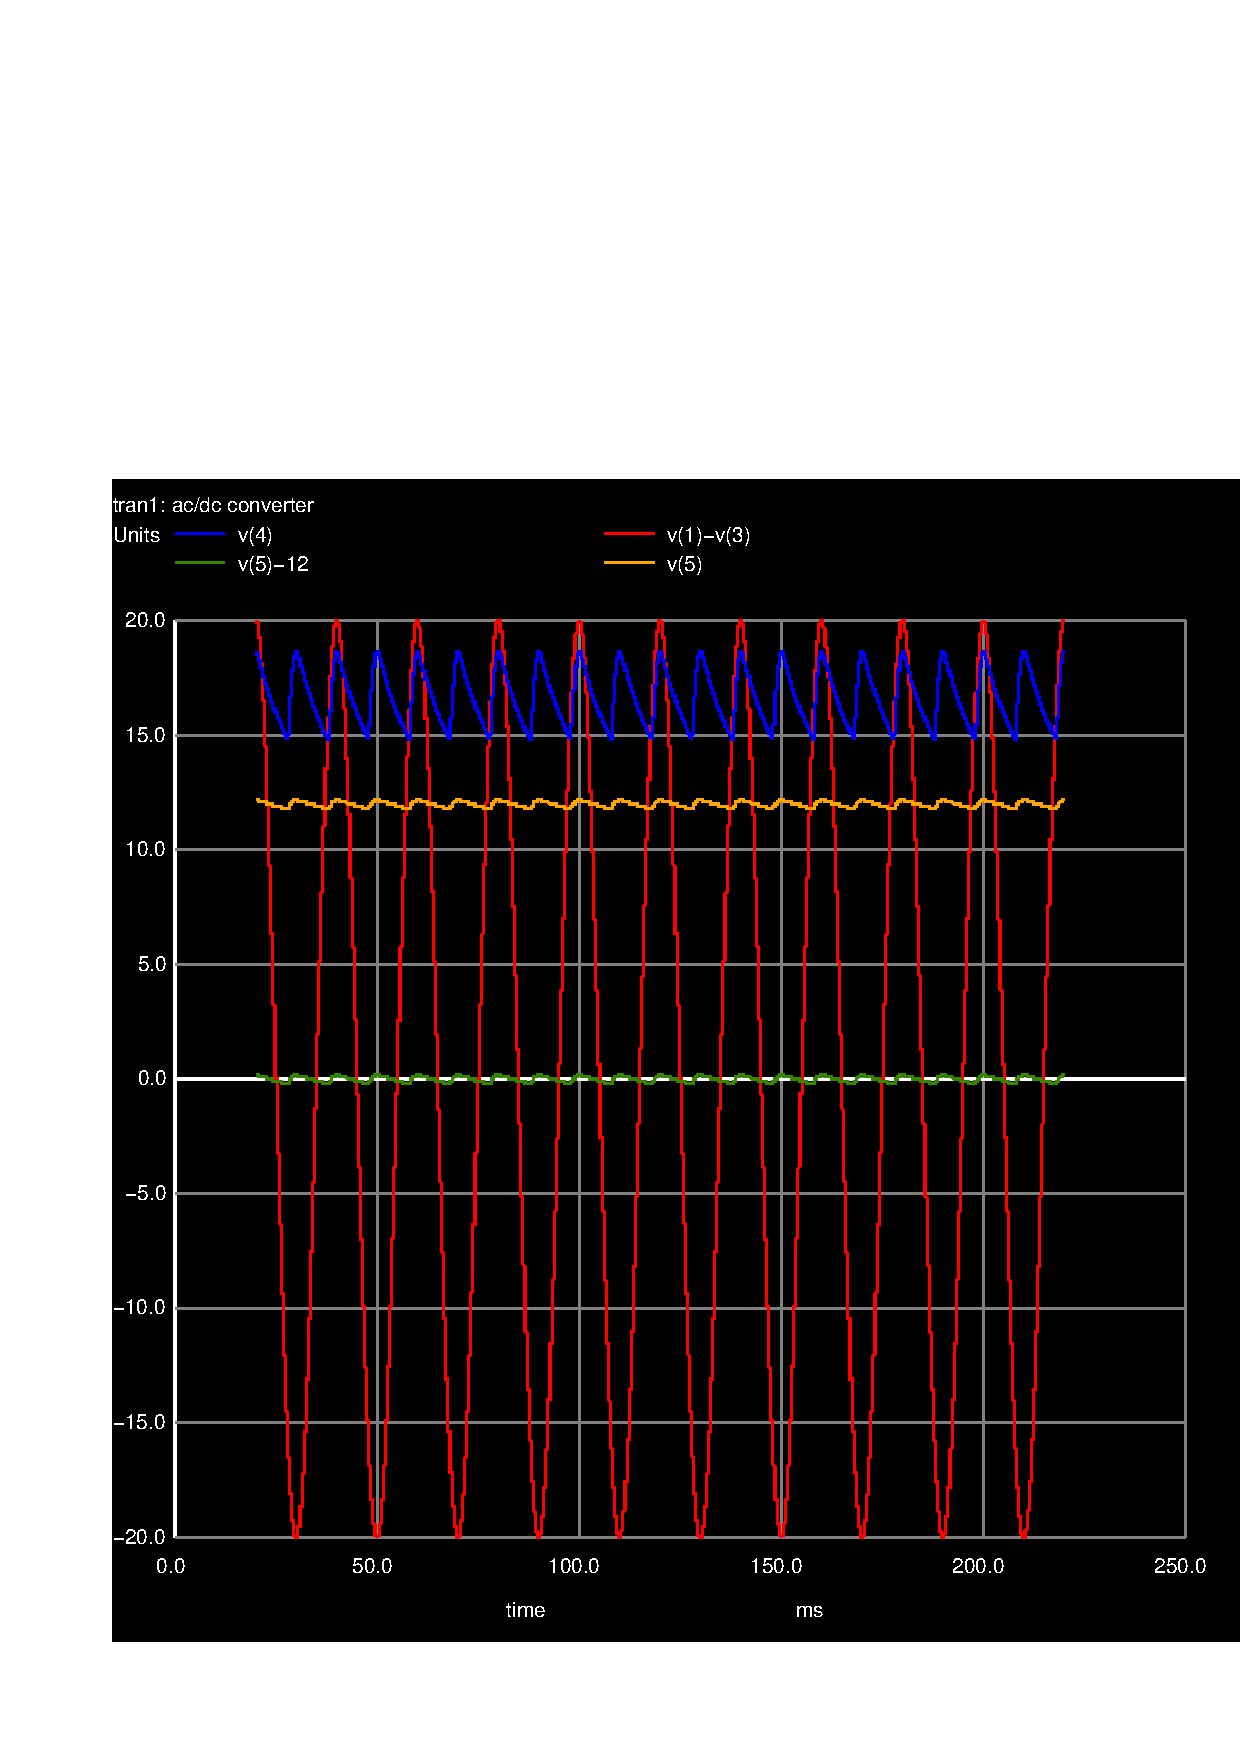
\includegraphics[width=0.6\linewidth]{vospice50.pdf}
\caption{Voltage simulation plots over time: red - voltage in secondary winding; blue - envelope detector output voltage; yellow - voltage regulator output voltage; green - ripple}
\label{fig:rc1}
\end{figure}

From Section ~\ref{sec:theo} we obtained one period of the waves, seen in Figures ~\ref{fig:vo} to ~\ref{fig:vofinal}. 

\begin{figure}[H] \centering
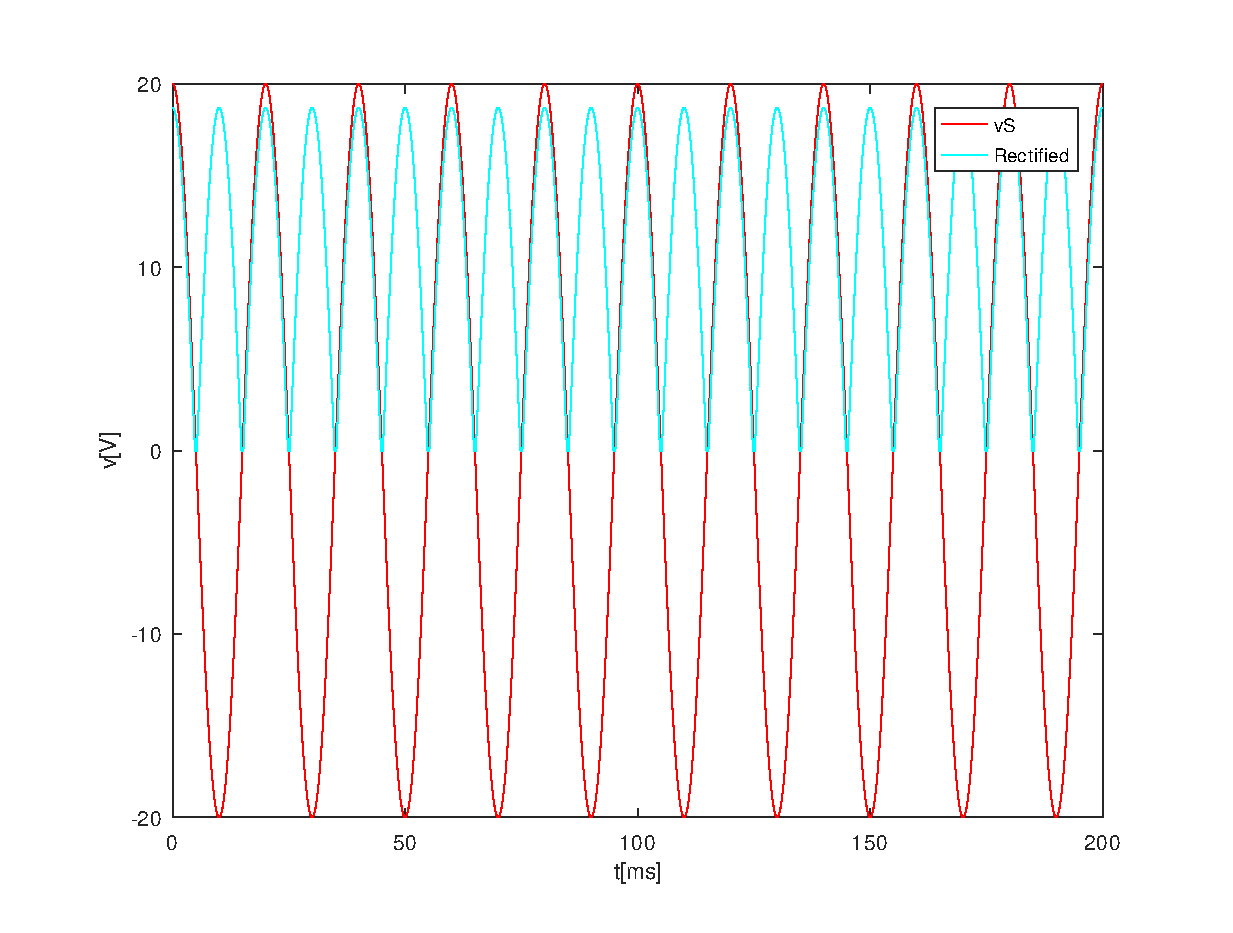
\includegraphics[width=0.4\linewidth]{vo.eps}
\caption{Voltage in the secondary winding (red) and voltage in rectifier (cyan) over time}
\label{fig:vo}
\end{figure}

\begin{figure}[H] \centering
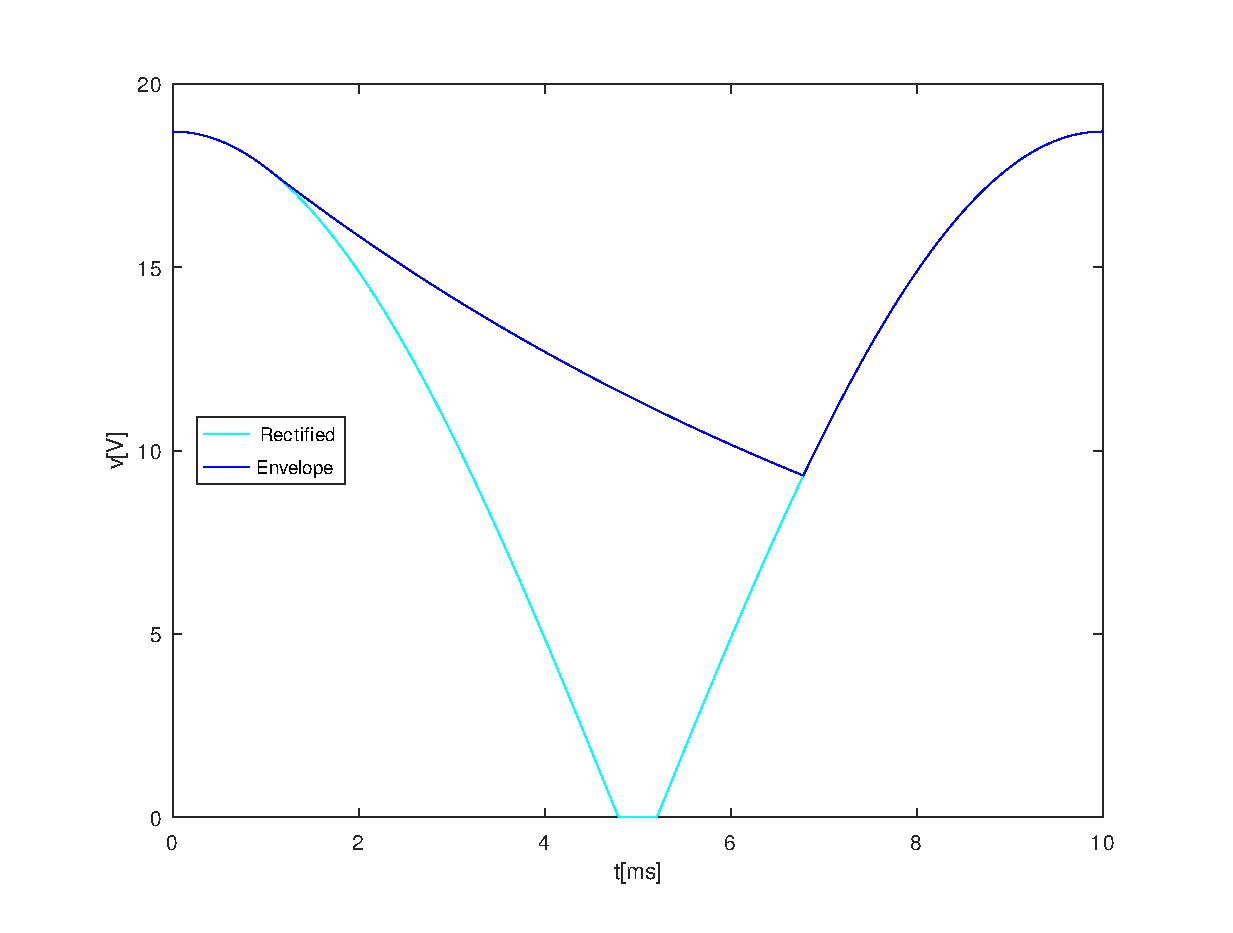
\includegraphics[width=0.4\linewidth]{venvlope.eps}
\caption{Envelope detector output voltage (blue) and voltage in rectifier (cyan) over one period}
\label{fig:voen}
\end{figure}

\begin{figure}[H] \centering
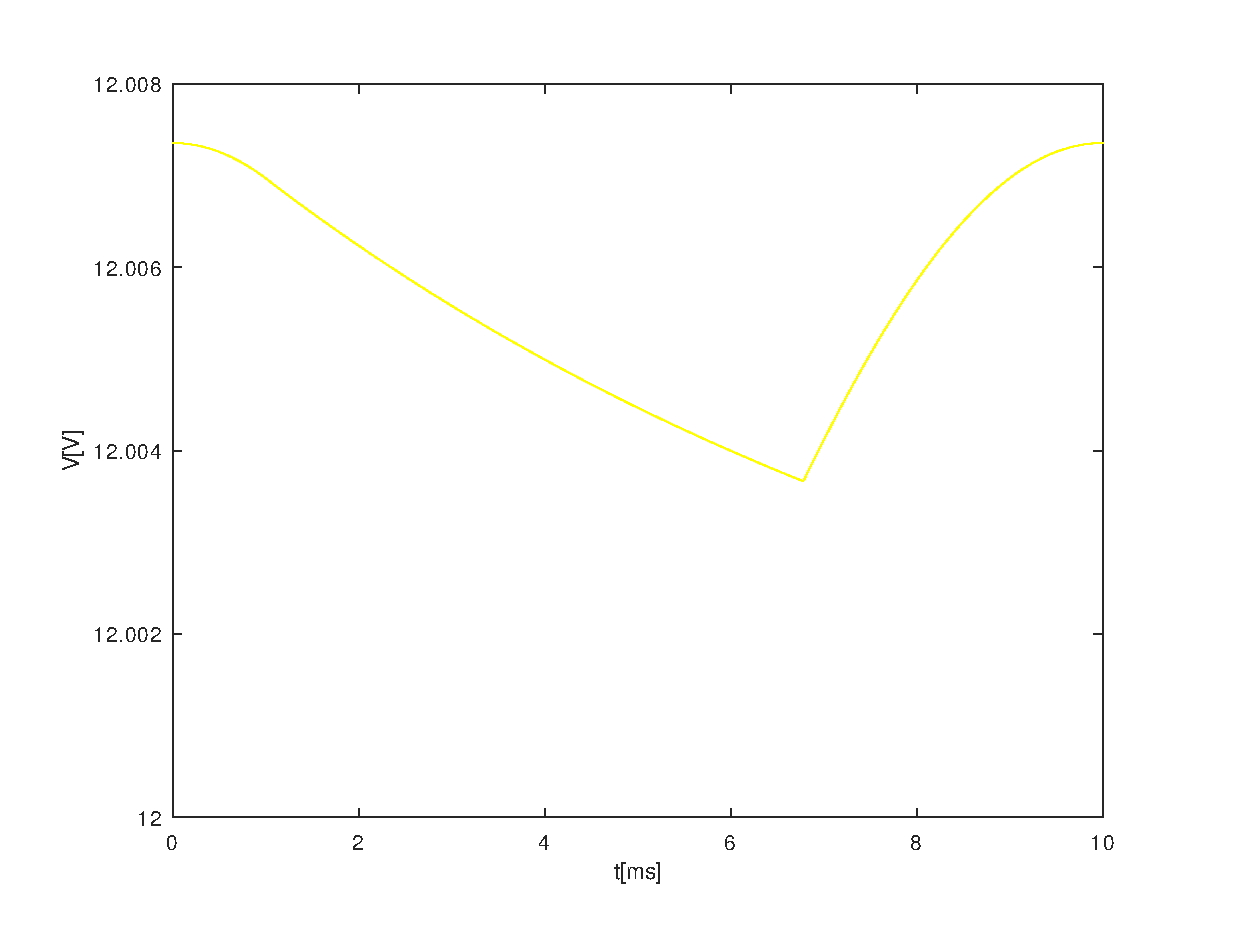
\includegraphics[width=0.4\linewidth]{vregulator.eps}
\caption{Voltage regulator output voltage over one period}
\label{fig:voreg}
\end{figure}

\begin{figure}[H] \centering
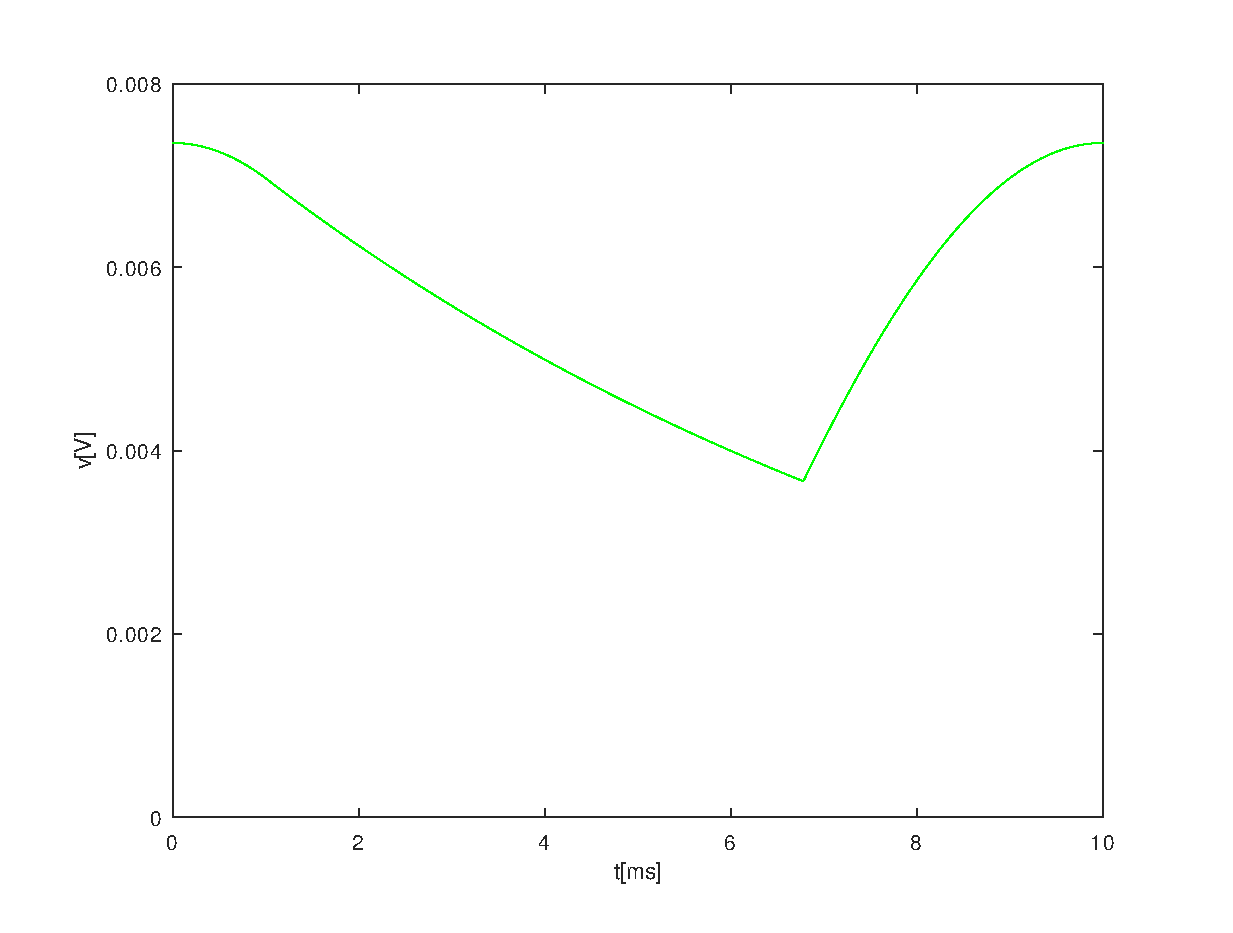
\includegraphics[width=0.4\linewidth]{vfinal.eps}
\caption{Ripple over one period}
\label{fig:vofinal}
\end{figure}

\subsection{Merit}
To calculate the merit we used the following equation:
\begin{equation}
M = \frac{1}{cost(ripple(v_O) + average(v_O - 12) + 10^{-6})}
\end{equation}
The cost is the sum of the cost of the resistor (1 MU/k$\Omega$), the capacitor (1 MU/$\mu$F) and the diodes (0.1 MU/diode). Our total cost is 8.2 MU.\\
The DC output level average was calculated using function average() in \textit{ngspice} and function mean() in \textit{octave}. The results were 11.99012V and 12.007V, respectively.\\
The ripple was calculated using functions max() and min() in both \textit{ngspice} and \textit{octave}. The results were 0.35752V and 0.00036995V, respectively.\\
The merit was only calculated for the \textit{ngspice} simulation and the result was 0.3319.

\section{Conclusions}
\label{sec:conc}
Our results were pretty consistent between the two analysis; the central frequencies were quite close (only around a 10Hz difference), the gain was exactly the same to the third decimal place and the plots of the frequency response were extremely similar, both displaying the same behaviour. \\
The subtle changes in the results can be explained by two facts. First of all in the theoretical model we consideral an ideal OPAMP so the gain is slightly larger in this analysis. Secondly, there are non-linear elements in the circuit (diodes, transistors, capacitors), these introduce some unexpected behaviour.\\
The differences in the phase plots are explained because in the ngspice simulation the OPAMP model has two internal capacitors, (2 poles). This causes a sudden shift in the phase of $\frac{\pi}{2}$ per pole, so it rises sharply $\pi$ radians.\\
The impedances again, are very consistent. The input impedance is large, as desired. The output impedance is a bit larger than expected, but it is still smaller and in another order of magnitude of the input impedance.\\
Finally, the merit calculated is quite low. This is a result of the high cost (especially taking into consideration the cost of the OPAMP). The gain deviation is also considerable, the central frequency deviation being the most successful.

%\cleardoublepage

% ----------------------------------------------------------------------
%  Bibliography
% ----------------------------------------------------------------------
%\addcontentsline{toc}{section}{\bibname}
%\bibliographystyle{abbrvunsrtnat} % <<<<< SELECT IF USING REFERENCES BY NUMBER (CITATION ORDER)
%\bibliography{../../../BIBfile.bib}

% ----------------------------------------------------------------------
\end{document}
% ----------------------------------------------------------------------

